{\color{indiagreen}\subsection{Editor}}
Kot vsako razvojno okolje ima tudi Unity 3D svoj privzeti editor. To je MonoDevelop, ki podpira večplatformski razvoj(to pomeni, da lahko isto kodo pišemo za različne operacijske sisteme Linux, Windows, Mac itd.). Podpira naslednje jezika: \\
\begin{itemize}
	\item C\#
	\item F\#
	\item VisualBasic
	\item \dots
\end{itemize}
Ima tudi integrirano dopolnjevanje kode(code auto-completion) in svoj debuger. Sam sem kar nekaj časa uporabljal MonoDevelop in v njemu razvijal, ampak mi pri je pri njem vedno nekaj manjkalo. Zdelo se mi je, da je njihov code auto-completion vsiljeval svoje stvari in da mi highliter ni vedno obarval kakšnih klasov. Zato sem se odločil, da bom začel uporabljati meni ljubši urejevalnik besedila to je Sublime Text 3. Pri tem urejevalniku sem dobil veliko svobodo pri urejanju, iskanju, popravljanju ter pri samem urejanju urejevalnika. To sublime omogoča s svojim Package Controlom, ki se ga da inštalirati preko te strani: \url{https://packagecontrol.io/installation}. Preko Package Controla lahko inštaliramo dodatne plugine in snippete za sublime, ki izboljšajo samo delovanje tega. O tej temi bi se dalo še veliko govoriti zato jo bom pustil za drugič. Seveda moramo Unityju povedati, da naj svoje datoteke odpira z sublimom. To naredimo tako:\\
\begin{enumerate}
	\item Inštaliramo Sublime Text 3/2 preko te \href{http://www.sublimetext.com/3}{strani}
	\item Gremo v \textbf{Edit} $\rightarrow$ \textbf{Preferences} $\rightarrow$ \textbf{External Tools}(kot lahko vidimo v spodnji sliki) in spremenimo na[ urejevalnik\\
	\begin{figure}[h]
  		\centering
		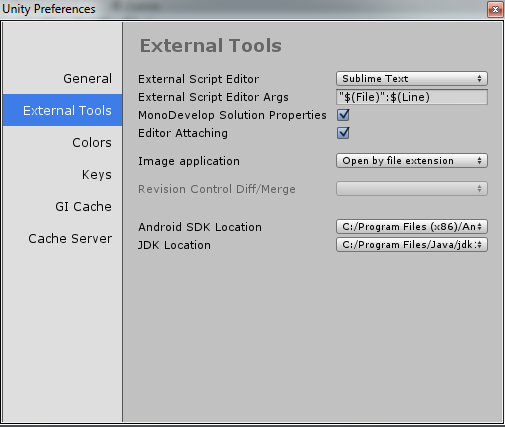
\includegraphics[width=15cm, height=15cm,keepaspectratio=true]{UnitySublime1.png}
		\caption{Sublime Text Set Up}
	\end{figure}
	\item Spremenimo \textbf{External Script Editor Args} v "\$(File)":\$(Line) zato, da bo sublime skočil v vrstico, kjer je error 
	\item Sedaj bi nam moral Unity odpreti sublime, ko dvokliknemo na datoteko, ki je skripta
	\item V sublimu bomo še spremenili, katere datoteke hočemo videti v projeknem drevesu. To naredimo tako, da gremo v \textbf{Project} $\rightarrow$ \textbf{Save Project As} in notri vtipkamo tole kodo:\\
	\begin{minted}[mathescape,
               linenos,
               numbersep=5pt,
               gobble=2,
               frame=lines,
               framesep=2mm]{json}
		{
			"folders":
			[
				{
					"path": "Assets/Scripts",
					"file_exclude_patterns":
					[
						"*.dll",
						"*.meta"
					]
				}
			]
		}
		
	\end{minted}
	in potem shranimo datoteko. To nam scrije vse nepotrebne .meta in .dll datoteke
	\item S Package Controlom na koncu še inštaliramo dodatne snippete, ki nam pomagajo pri auto-completion in barvanju kode. Vse potrebne package najdemo na tej strani \url{http://wiki.unity3d.com/index.php/Using_Sublime_Text_as_a_script_editor}, kjer so tudi bolj podrobna navodila za celoten setup Sublime Text-a.
\end{enumerate}
Kot zanimivost pa bi vam rad pokazal, kako enostavno se da narediti snippete v Sublime Text-u, ki se potem sprožijo ob določenem zaporedju tipk in nakoncu tabulatorja. 
\begin{minted}[mathescape,
           linenos,
           numbersep=5pt,
           gobble=2,
           frame=lines,
           framesep=2mm]{json}
	{
		"folders":
		[
			{
				"path": "Assets/Scripts",
				"file_exclude_patterns":
				[
					"*.dll",
					"*.meta"
				]
			}
		]
	}
	
\end{minted}